\chapter{Background\label{cha:chapter2}}

This chapter covers the basic concepts crucial for understanding this thesis, providing the essential information, without having a deep explanation of each topic.

\section{Blockchain}

A blockchain consists of a distributed ledger that maintains an ever-expanding series of records (\textit{blocks}), interconnected through cryptographic hashes, where a block contains multiple transactions. In addition to the transactions, each block stores a timestamp, the hash value of the previous block (\textit{parent}) and a nonce, which is a random number used to verify the hash. This concept ensures the integrity of the entire blockchain through the first block, called \textit{genesis block}. Hash values are unique and fraud can be successfully prevented since changes of a block in the chain would immediately change the respective hash value. This setup allows for the construction of a chain-like structure (similar to a linked list data structure), where every new block is connected to the previous. Due to this structure, modifying information within a specific block after it's published isn't feasible without modifying all subsequent blocks, making blockchain transactions irreversible. \cite{nofer_blockchain_2017}

The operation of blockchains usually takes place on a peer-to-peer network. In this network, nodes collaborate following a consensus algorithm protocol to include and verify new blocks. Blockchains are often perceived as secure, while it's known that blockchain records might not be entirely immutable due to the potential of blockchain forks: cases when two valid blocks with the same parent are produced and two valid branch co-exist for a short period of time \cite{goldberg_short_2019}.

\subsection{Tezos}

Tezos \cite{allombert_introduction_2019} is a relatively new blockchain, based on the proof-of-stake consensus. The main proprieties of this blockchain are:
\begin{itemize}
      \item \textbf{Self amending blockchain}: the protocol that validates blocks and implements the consensus algorithm can amend itself;
            \vspace{-0.11in}
      \item \textbf{Proof-of-stake}: it considers the stake (the number of tokens) that users hold as the primary resource used to build the pool of block producers;
            \vspace{-0.11in}
      \item \textbf{Formal verification}: the code base is mainly written in the OCaml programming language, whose robust static type system and memory management system rule out many common runtime errors like null pointer exceptions or buffer overflows.
\end{itemize}

Tezos' smart contract language is Michelson. It is very low level, comparable to Assembly: for this reason there are several high level languages that compile to Michelson, like Ligo and SmartPy.

\section{Hash Function \& Merkle Tree}

A hash function is a fundamental cryptographic tool. A one way hash function F is one which is easy to compute but difficult to invert and can map arbitrarily large data fields onto much smaller ones. If $y = F(x)$, then given $x$ and $F$, it is easy to compute $y$, but given $y$ and $F$ it is effectively impossible to compute $x$ \cite{merkle_secrecy_1979}. Many implementations exist, varying by the collision resistance property, performance, and security. Some of the most used hash functions are MD5, sha2 family and sha3.

A possible application of one way hashing function useful for this master thesis is the Merkle Tree. Merkle Trees have been introduced in \cite{merkle_secrecy_1979} and consist in binary trees, where leafs are simple raw data, and the nodes are the one way hash of the two child subtrees roots. This structure allows to verify the integrity of the data, storing only a single hash. In fact, if the root hash is known, it's possible to verify if a specific data is part of the tree, by recomputing the Merkle Tree and comparing the computed root hash with the one stored.

In recent times new Hash functions have been designed in order to be more efficient when executed in a Zero Knowledge environment. \cite{grassi_poseidon_2021} is one of the most recent and efficient one: it is considered a `sponge hash' because has a variable number of inputs and outputs, depending on the environment where the hash function is executed. It allows for a minimal complexity increase for each hash executed when compiled in a zero knowledge environment. It can perform 200 times more efficiently than the sha256 hash function and allows for a customization of security and throughput based on the needs.

\section{Zero Knowledge Proofs \& zkSnark}

The concept of a `proof system of possession of knowledge' represents a protocol between two parties called the prover and the verifier where the prover wants to convince the verifier that he knows the proof of a given theorem \cite{de_santis_zero-knowledge_1992}. This technology has been studied since the '80s, but is finding a broad application nowadays in the blockchain field. A more recent application of Zero knowledge Proofs is zk-SNARK \cite{bitansky_extractable_2012}. It allows a proof generation from an execution of a program, and a verification of the proof without the need of the program nor the inputs and outputs. zkSNARKs have valuable proprieties, effectively composing the zkSNARK name:
\begin{itemize}
      \item \textbf{Succinct}: the proof size is independent from the amount of computation done in the program;
            \vspace{-0.11in}
      \item \textbf{Non-interactive}: the proof can be verified without interaction with the prover;
            \vspace{-0.11in}
      \item \textbf{Argumented knowledge}: the proof statement is correct with non-negligible probability.
            \vspace{-0.11in}
\end{itemize}

\section{ZoKrates}

ZoKrates is a toolbox for zkSNARKs on Ethereum: it allows developers to write zero-knowledge proofs in a high-level programming language and generate trusted setup parameters and zero-knowledge proofs \cite{eberhardt_ZoKrates_2018}. In the case of SNARK proofs it is in fact necessary to rely on a trusted setup phase to generate the proving and verification keys, which are used to generate and verify the proofs.

This toolbox utilizes a language style similar to C++, facilitating developers adoption. It also offers a built-in library with frequently used functions like hash functions, elliptic curve operations, and Merkle tree operations. The toolbox is also capable of generating a Solidity contract from the ZoKrates program, deployable on the Ethereum blockchain, to allow verification of proofs on chain. The contract can then be used to verify the proofs generated by the ZoKrates program. However, a drawback of this toolbox is the limited supported data types: due to the resource-intensive phases like computing the witness and generating a proof, the program must avoid using complex and memory-consuming types. For this reason the primitive types supported are integers, booleans and field values, whose size depends on the underlying elliptic curve.

Another constraint is that the toolbox requires loop sizes to be known during compile time. This becomes problematic when dealing, for instance, with a variable number of users, as the number of iterations of the loops depends on the number of users.

ZoKrates produces verifiable proofs, defined as follows: a structure with proof keys, public program inputs and program outputs. It's generated using a proving key and can be verified only using the corresponding verification key.

Figure \ref{fig:2_zokrates-flow} shows the sequence of ZoKrates phases execution. The phases marked with a circle are done only once during the lifetime of a program, while the ones marked with a square are executed for each program execution.

\begin{figure}[htb]
      \centering
      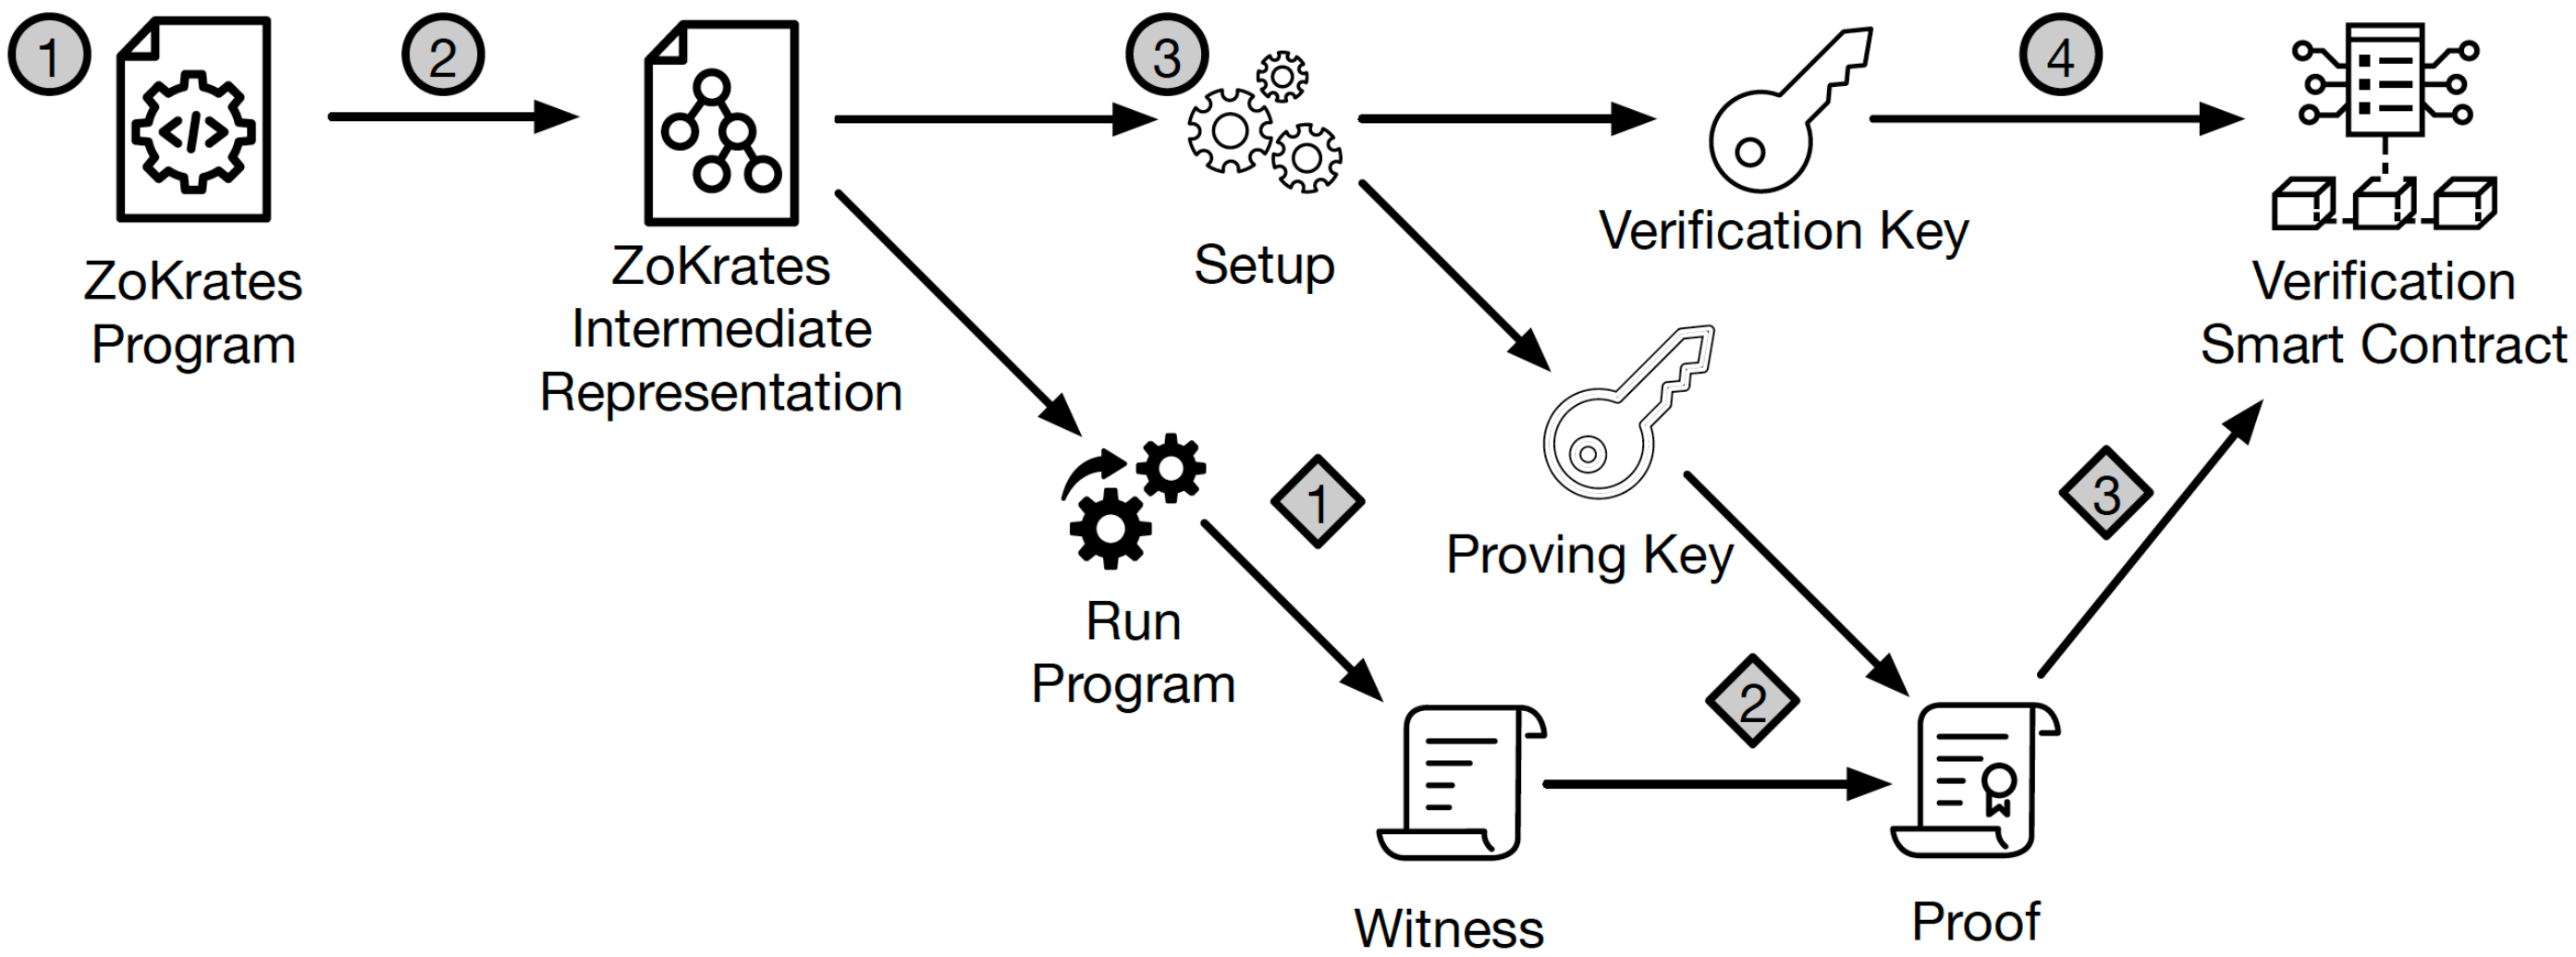
\includegraphics[width=0.8\columnwidth]{2_zokrates-flow.png}
      \caption{ZoKrates Phases \cite{ise_department_tub_material_nodate}}
      \label{fig:2_zokrates-flow}
\end{figure}

\section{Signature \& BLS12-381}

A signature is a mathematical scheme for demonstrating the authenticity of a digital message or document. A valid digital signature gives a recipient reason to believe that the message was created by a known sender, and that it was not altered in transit. This mechanism allows a system to receive some messages and be confident that they are authentic, even if the sender can not be trusted. Signatures are heavily dependant on the hash function used, and the curve on which the signature is generated.

The curve BLS12-381\footnote{\url{https://electriccoin.co/blog/new-snark-curve/}} has been developed to be friendly with technologies like zkSNARKs, and is currently supported by Tezos and ZoKrates, allowing the verification of proofs on-chain.